
\maketitle

Student Name: \hfill Student Email: \hspace{10em}
\section{Instructions}
\begin{itemize}
  \item Time allowed is 50 minutes. (This sample exam might be lengthier than the actual exam. )
  \item In order to minimize distraction to your fellow students, you may not leave
  during the last 10 minutes of the examination.
  \item The examination is closed-book. One 8x11in cheatsheet is allowed.
  \item Non-programmable calculators are permitted.
  \item The maximum number of marks is 100, as indicated; the midterm examination
  amounts 10\% toward the final grade.
  \item Please use a pen or heavy pencil to ensure legibility.
  \item Please show your work; where appropriate, marks will be awarded for proper and well-reasoned explanations.
\end{itemize}

\begin{prob}
  Number conversions:
  \begin{enumerate}
    \item Use repeated division to convert $230_{10}$ to octal representation (5 marks).
    \item What is the value of $19D_{16}$ in base 10 (5 marks).
    \item A 6-bit two's complement number is $100011_{2}$. Convert it to (signed) decimal (5 marks).
    \item Represent $-23_{10}$ in two's complement binary notation (5 marks).
  \end{enumerate}
\end{prob}

\begin{prob}
  Consider the circuit below\\
  \begin{tikzpicture}[circuit logic US]
    \matrix[column sep=7mm]
    {
      \node (A) {A}; &  &  & \\
      & \node [xor gate] (AxorB) {}; &  &\\
      \node (B) {B}; &  & \node [xor gate] (f) {}; \\
      & \node [xor gate] (BxorC) {}; &  & \\
      \node (C) {$\bC$}; &  & &\\
    };
    \draw (A.east) --++(right:3mm) |- (AxorB.input 1);
    \draw (B.east) --++(right:3mm) |- (AxorB.input 2);
    \draw (A.east) --++(right:1mm) |- (BxorC.input 1);
    \draw (C.east) --++(right:3mm) |- (BxorC.input 2);
    \draw (AxorB.output) to [edge label=$g_1$] ++(right:3mm) |- (f.input 1);
    \draw (BxorC.output) to [edge label=$g_2$] ++(right:3mm) |- (f.input 2);
    \draw (f.output) to [edge label=Y] ++(right:3mm) ;
  \end{tikzpicture} \\
  By algebraic manipulation, prove or disprove that $Y = \bB \bC + B C$ (10 marks).
\end{prob}

\begin{prob}
Use the following 5-variable K-map for F (A, B, C, D, E), and find
  a minimal SOP expression for F (15 marks)\\
\begin{minipage}{0.5\linewidth}
  \centering
  \begin{Karnaugh}{BC}{DE}
    \minterms{0,1,5,6,7,8,9,14}
  \end{Karnaugh}\\
  A=0
\end{minipage}%
\begin{minipage}{0.5\linewidth}
  \centering
  \begin{Karnaugh}{BC}{DE}
    \minterms{1,4,5,6,7,9,12,14}
  \end{Karnaugh}\\
  A=1
\end{minipage}
\end{prob}

\begin{prob}
  Use bubble-pushing and/or algebra to find an SOP expression
for Y in the circuit below. If you use bubble-pushing, draw an equivalent
  circuit beside the given circuit (5 marks).\\
  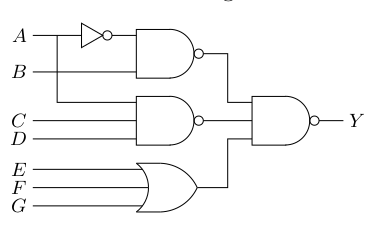
\includegraphics[width=0.4\linewidth]{figures/bubble-pushing-circuit.png}
\end{prob}

\begin{prob}
  Consider the function Y given below.
  \[ Y(A, B, C, D) = \sum m(0, 3, 5, 7, 8, 14) + d(2, 12, 15) \]
  \begin{enumerate}
    \item Draw a K-maps to derive a minimum SOP and POS expressions for Y .
      Indicate all essential prime implicants for Y or $\bY$ in your K-maps (20 marks).
    \item Sketch a two-level NOR-NOR circuit for Y. Assume that A, B, C, and D are available in true end complimentary forms (5 marks).
    \item Write Y in Product of sums (POS) \emph{canonical} form (5 marks).
  \end{enumerate}
\end{prob}

\begin{prob}
  Design a minimal SOP circuit to add two two-bit unsigned numbers. Denote the two bits of first number as $A_1A_0$ and the two bits of second number as $B_1B_0$. The result will be a 2-bit sum $S_1S_0$ and a carry $C$. Start with filling out the following truth table (3 example rows are provided) and then use K-maps to find minimal SOP for $S_1$, $S_0$ and a single carry bit $C_1$ (20 marks).
  \begin{tabular}{cccc|ccc}
    \toprule
    $A_1$ & $A_0$ & $B_1$ & $B_0$ & $C_1$ & $S_1$ & $S_0$  \\
    \midrule
    0 & 0 & 0 & 0 &   &   &   \\
    0 & 0 & 0 & 1 &   &   &   \\
    0 & 0 & 1 & 0 &   &   &   \\
    0 & 0 & 1 & 1 &   &   &   \\
    0 & 1 & 0 & 0 &   &   &   \\
    0 & 1 & 0 & 1 & 0 & 1 & 0 \\
    0 & 1 & 1 & 0 &   &   &   \\
    0 & 1 & 1 & 1 &   &   &   \\
    1 & 0 & 0 & 0 &   &   &   \\
    1 & 0 & 0 & 1 &   &   &   \\
    1 & 0 & 1 & 0 &   &   &   \\
    1 & 0 & 1 & 1 &   &   &   \\
    1 & 1 & 0 & 0 &   &   &   \\
    1 & 1 & 0 & 1 & 1 & 0 & 0 \\
    1 & 1 & 1 & 0 &   &   &   \\
    1 & 1 & 1 & 1 & 1 & 1 & 0 \\
    \bottomrule
  \end{tabular}
\end{prob}
